\documentclass[10pt]{article}
\usepackage[utf8]{inputenc}
\usepackage[doublespacing]{setspace}
\usepackage{textcomp}
\usepackage{amsmath,amssymb,amsthm}
\usepackage{fancyhdr}
\usepackage{lastpage}
\usepackage[]{hyperref}
\usepackage[pdftex]{graphicx}
\usepackage{ctex}
\usepackage{booktabs}
\usepackage{subfigure}
\usepackage{titlesec}
\usepackage{listings}
\usepackage{enumerate}
\usepackage{bm}
\usepackage{float}
\usepackage{url}
\usepackage[english]{babel}
\usepackage[dvipsnames]{xcolor}
%\allowdisplaybreaks
\renewcommand{\contentsname}{\centerline{Contents}}
\pagestyle{fancy}
\author{D}
\def\name{D}
\lhead{Multivariate Statistical Methods}
\chead{}
\rhead{\name}
\cfoot{-\space\thepage\space-}
\newtheorem{exer}{\bm{$Exercise$}}
\newtheorem{prob}{\bm{$Problem$}}
\newtheorem{bonus}{\bm{$Bonus\;Problem$}}
\newcommand{\tabincell}[2]{\begin{tabular}{@{}#1@{}}#2\end{tabular}}
\CTEXoptions[today=old]

\begin{document}

\title{Assignment One}
\date{\today}
\maketitle
\thispagestyle{fancy}
\thispagestyle{fancy}

\newpage

\begin{prob}
\end{prob}
\begin{enumerate}[1)]
\vspace{3mm}

\item
The assignment mark is the most useful for predicting final exam marks, with the correlation being 0.5803460; the test mark is the second most useful, with the correlation being 0.5735629.
\begin{table}[H]
\centering
\tiny
\begin{tabular}{lllllll}
           & Assignment & S1         & S2         & Project    & Test       & Exam      \\
Assignment & 1.0000000  & 0.39482004 & 0.5810368  & 0.3722818  & 0.3839863  & 0.5803460 \\
S1         & 0.39482004 & 1.0000000  & 0.21743378 & 0.17247814 & 0.09490252 & 0.1613426 \\
S2         & 0.5810368  & 0.21743378 & 1.0000000  & 0.2187980  & 0.1826170  & 0.4567156 \\
Project    & 0.3722818  & 0.17247814 & 0.2187980  & 1.0000000  & 0.26984593 & 0.3347456 \\
Test       & 0.3839863  & 0.09490252 & 0.1826170  & 0.26984593 & 1.0000000  & 0.5735629 \\
Exam       & 0.5803460  & 0.1613426  & 0.4567156  & 0.3347456  & 0.5735629  & 1.0000000
\end{tabular}
\caption{Correlation matrix}
\end{table}
\begin{figure}[H]
  \centering
  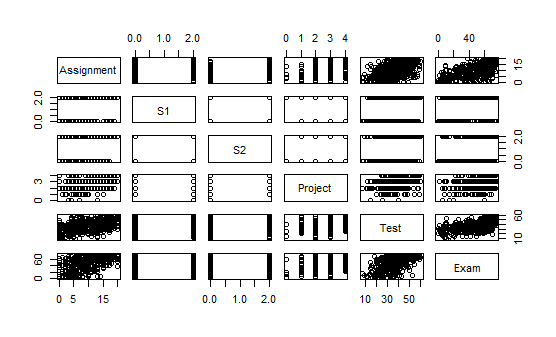
\includegraphics[scale=0.45]{p11a.png}
  \caption{Matrix plot}
\end{figure}

\item
Yes, the boxplots show that the mean of test marks for students who attend 75\% of the S1 tutes is approximately 7 higher than that of those for whom did not, and the distances between the first quarter and the mean and the third quarter and the mean look similar. This implies weak positive correlation.
\begin{figure}[H]
  \centering
  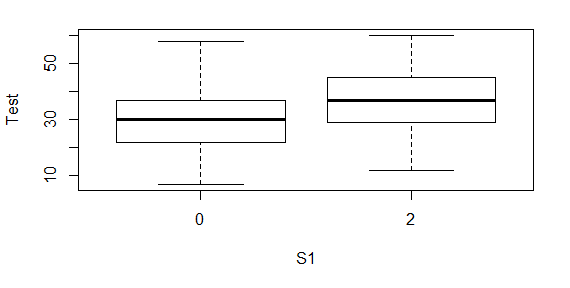
\includegraphics[scale=0.45]{p12a.png}
  \caption{Boxplot}
\end{figure}

\item
Yes. Since the assignment mark and test mark both have moderately strong positive correlation with the exam mark, the students with low assignment marks, low test marks and high exam marks as well as the students with high assignment marks, high test marks and low exam marks, which indicate negative correlation, can be considered unusual.
\begin{figure}[H]
  \centering
  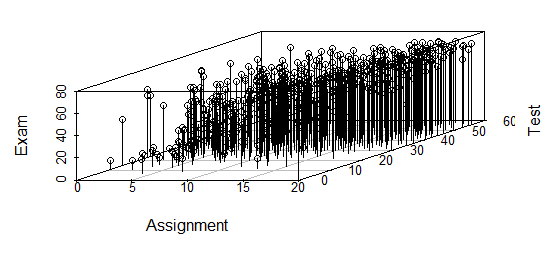
\includegraphics[scale=0.45]{p13a.png}
  \caption{3D scatterplot}
\end{figure}

\item
The observed association between the exam mark and the test mark includes moderately strong correlation and positive direction, implied by 0.5735629 correlation, and moderate non-linear relation, implied by the bow-shape graph; the observed association between the exam mark and the assignment mark includes moderately strong correlation and positive direction, implied by 0.5803460 correlation, and moderate non-linear relation, implied by the bow shape and the observed cluster in the top of the graph.
\begin{figure}[H]
  \centering
  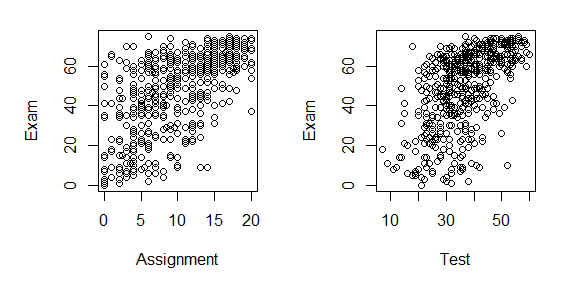
\includegraphics[scale=0.45]{p14a.png}
  \caption{2D scatterplots}
\end{figure}

\end{enumerate}
\vspace{3mm}

\newpage

\begin{prob}
\end{prob}
\vspace{3mm}

\begin{table}[H]
\centering
\tiny
\begin{tabular}{lllllll}
       & REACT                 & HEIGHT                & WEIGHT               & SHLDR                & PELVIC              & CHEST                 \\
REACT  & 1.00000000            & 0.2223465             & 0.05623396           & -0.09378423          & -0.05588815         & -0.031815353          \\
HEIGHT & 0.22234647            & 1.0000000             & \textbf{0.63533800}  & \textbf{0.65429474}  & \textbf{0.58589320} & \textbf{0.425921567}  \\
WEIGHT & 0.05623396            & \textbf{0.6353380}    & 1.00000000           & \textbf{0.66561662}  & \textbf{0.64701674} & \textbf{0.888689237}  \\
SHLDR  & -0.09378423           & \textbf{0.6542947}    & \textbf{0.66561662}  & 1.00000000           & \textbf{0.58243744} & \textbf{0.554491326}  \\
PELVIC & -0.05588815           & \textbf{0.5858932}    & \textbf{0.64701674}  & \textbf{0.58243744}  & 1.00000000          & \textbf{0.522053941}  \\
CHEST  & -0.03181535           & \textbf{0.4259216}    & \textbf{0.88868924}  & \textbf{0.55449133}  & \textbf{0.52205394} & 1.000000000           \\
THIGH  & 0.13240364            & 0.2231891             & \textbf{0.55421714}  & 0.20457158           & 0.20749443          & 0.397798097           \\
PULSE  & 0.16311131            & -0.1815138            & -0.26384261          & -0.16823801          & -0.32294930         & -0.246277838          \\
DIAST  & 0.14731786            & -0.1865544            & -0.05169953          & -0.14487864          & 0.14774246          & -0.008424785          \\
CHNUP  & -0.15846427           & -0.2760095            & \textbf{-0.57578361} & -0.27386998          & -0.15815654         & \textbf{-0.453590531} \\
BREATH & 0.15952838            & \textbf{0.5878336}    & \textbf{0.45020129}  & 0.36765212           & 0.35357088          & 0.347296368           \\
RECVR  & -0.12957499           & -0.1212571            & -0.12188067          & -0.02394390          & -0.20686139         & -0.083230108          \\
SPEED  & -0.14933515           & 0.2156329             & -0.05264149          & 0.20175308           & 0.04123524          & -0.162411673          \\
ENDUR  & -0.05254842           & -0.1891603            & -0.36798260          & -0.24477548          & -0.22935383         & -0.327536559          \\
FAT    & 0.16480503            & 0.3651088             & \textbf{0.80950678}  & 0.33062913           & \textbf{0.41321623} & \textbf{0.724615152}  \\
       & THIGH                 & PULSE                 & DIAST                & CHNUP                & BREATH              & RECVR                 \\
REACT  & 0.132403643           & 0.163111309           & 0.147317859          & -0.15846427          & 0.15952838          & -0.12957499           \\
HEIGHT & 0.223189118           & -0.181513836          & -0.186554416         & -0.27600951          & \textbf{0.58783355} & -0.12125711           \\
WEIGHT & \textbf{0.554217142}  & -0.263842612          & -0.051699534         & \textbf{-0.57578361} & \textbf{0.45020129} & -0.12188067           \\
SHLDR  & 0.204571577           & -0.168238013          & -0.144878644         & -0.27386998          & 0.36765212          & -0.02394390           \\
PELVIC & 0.207494435           & -0.322949297          & 0.147742457          & -0.15815654          & 0.35357088          & -0.20686139           \\
CHEST  & 0.397798097           & -0.246277838          & -0.008424785         & \textbf{-0.45359053} & 0.34729637          & -0.08323011           \\
THIGH  & 1.000000000           & -0.006222473          & 0.048680731          & \textbf{-0.66952595} & 0.20652250          & 0.20312822            \\
PULSE  & -0.006222473          & 1.000000000           & 0.234087585          & 0.15477615           & -0.06435685         & \textbf{0.50389072}   \\
DIAST  & 0.048680731           & 0.234087585           & 1.000000000          & 0.05374787           & -0.16483499         & 0.15383829            \\
CHNUP  & \textbf{-0.669525949} & 0.154776147           & 0.053747870          & 1.00000000           & -0.35762039         & -0.06024670           \\
BREATH & 0.206522496           & -0.064356846          & -0.164834990         & -0.35762039          & 1.00000000          & 0.09127839            \\
RECVR  & 0.203128223           & \textbf{0.503890717}  & 0.153838286          & -0.06024670          & 0.09127839          & 1.00000000            \\
SPEED  & -0.208038863          & -0.299576960          & -0.320921118         & 0.32389717           & -0.03121830         & \textbf{-0.43651538}  \\
ENDUR  & -0.335725404          & 0.007295956           & 0.133656489          & 0.21277543           & -0.31457144         & -0.07279508           \\
FAT    & \textbf{0.844206678}  & -0.094830152          & 0.044647101          & \textbf{-0.69116892} & 0.29870144          & 0.06651871            \\
       & SPEED                 & ENDUR                 & FAT                  &                      &                     &                       \\
REACT  & -0.14933515           & -0.052548416          & 0.16480503           &                      &                     &                       \\
HEIGHT & 0.21563288            & -0.189160280          & 0.36510876           &                      &                     &                       \\
WEIGHT & -0.05264149           & -0.367982602          & \textbf{0.80950678}  & \textbf{}            &                     &                       \\
SHLDR  & 0.20175308            & -0.244775482          & 0.33062913           &                      &                     &                       \\
PELVIC & 0.04123524            & -0.229353829          & \textbf{0.41321623}  & \textbf{}            &                     &                       \\
CHEST  & -0.16241167           & -0.327536559          & \textbf{0.72461515}  & \textbf{}            &                     &                       \\
THIGH  & -0.20803886           & -0.335725404          & \textbf{0.84420668}  & \textbf{}            &                     &                       \\
PULSE  & -0.29957696           & 0.007295956           & -0.09483015          &                      &                     &                       \\
DIAST  & -0.32092112           & 0.133656489           & 0.04464710           &                      &                     &                       \\
CHNUP  & 0.32389717            & 0.212775434           & \textbf{-0.69116892} &                      &                     &                       \\
BREATH & -0.03121830           & -0.314571443          & 0.29870144           &                      &                     &                       \\
RECVR  & \textbf{-0.43651538}  & -0.072795081          & 0.06651871           &                      &                     &                       \\
SPEED  & 1.00000000            & -0.022480788          & -0.20551431          &                      &                     &                       \\
ENDUR  & -0.02248079           & 1.000000000           & \textbf{-0.40546220} & \textbf{}            &                     &                       \\
FAT    & -0.20551431           & \textbf{-0.405462200} & 1.00000000           &                      &                     &
\end{tabular}
\caption{Correlation matrix}
\end{table}

% In the correlation matrix, the values greater than 0.4 are printed in bold texts.\\
We partition the variables into subgroups. Firstly, the greatest correlation magnitude is 0.88, indicating the correlation between CHEST (min chest circumference) and WEIGHT. The correlation between WEIGHT and FAT (total body fat) is 0.80 and the correlation between CHEST and FAT is 0.72. All these magnitudes are great, so these three variables should be in the same subgroup. It is understandable in physical meanings that the higher weight a person has, the more fat his or her body stores, and the bigger his or her chest is. Secondly, some other related variables can be in this subgroup. The correlations between PELVIC (width of pelvic) and WEIGHT, CHEST and FAT are 0.64, 0.52 and 0.41 respectively. The weight of one's pelvic should be positively correlated with his or her weight. The correlations between SHLDR (shoulder width) and WEIGHT, PELVIC and CHEST are 0.66, 0.58 and 0.55 respectively. The correlations between HEIGHT and WEIGHT, SHLDR, PELVIC and CHEST are 0.63, 0.65, 0.58 and 0.42 respectively. The weight as well as other body size variables is positively correlated with one's shoulder width and height. The correlations between CHNUP (number of chin-ups completed in 1 min) and WEIGHT, CHEST and FAT are -0.57, -0.45 and -0.69 respectively. Usually people with lower weight and less fat can do more chin-ups. The correlations between THIGH (thigh skinfold thickness) and WEIGHT, CHNUP and FAT are 0.55, -0.66 and 0.84. These variables should be in the subgroup as well. The thigh skinfold thickness is highly correlated with one's fat. The correlations between BREATH (max breathing capacity) and WEIGHT and SHLDR are 0.58783355 and 0.45. The person with a bigger body size probably has bigger breathing capacity. This subgroup represents one's body measurement. Thirdly, PULSE (resting pulse rate), RECVR (pulse rate after 5 min recovery from treadmill) and SPEED (maximum treadmill speed) can be in the second subgroup, for the correlation between PULSE and RECVR is 0.50 and the correlation between SPEED and RECVR is -0.43. Both PULSE and RECVR are about pulse rates and one's treadmill speed probably may be related to them. This subgroup represents one's athletic index. Lastly, the remained variables are in each individual subgroup. REACT (reaction time to visual stimulus) that has small correlation magnitudes with any other variable is in the third subgroup. DIAST (diastolic blood pressure) is in the fourth subgroup. ENDUR (treadmill endurance time) is in the fifth subgroup. These subgroups represent other miscellaneous measurements. In all, the final groups of variables are:\\
Group 1: HEIGHT, WEIGHT, SHLDR, PELVIC, CHEST, THIGH, CHNUP, BREATH and FAT;\\
Group 2: PULSE, RECVR and SPEED;\\
Group 3: REACT;\\
Group 4: DIAST;\\
Group 5: ENDUR.
\vspace{3mm}

\begin{prob}
\end{prob}
\vspace{3mm}

(Both my solutions to 3.b and 3.a are presented, printed in black and gray respectively. Please grade 3.b.)\\

b)

\begin{enumerate}[1)]
\item
Assume \textbf{X} is a matrix, where
\[
\textbf{X}=
  \begin{bmatrix}
    x_{11} & x_{12} & \dots & x_{1p}\\
    x_{21} & x_{22} & \dots & x_{2p}\\
    \vdots & \vdots & \ddots & \vdots\\
    x_{n1} & x_{n2} & \dots & x_{np}
  \end{bmatrix}
.
\]
Then we get its transpose,%\footnote{\;\textbf{X\textsuperscript{T}} denotes the transpose of a matrix \textbf{X} and is equivalent to \textbf{X\textsuperscript{$\prime$}}.}
\[
\textbf{X\textsuperscript{$\prime$}}=
  \begin{bmatrix}
    x_{11} & x_{21} & \dots & x_{n1}\\
    x_{12} & x_{22} & \dots & x_{n2}\\
    \vdots & \vdots & \ddots & \vdots\\
    x_{1p} & x_{2p} & \dots & x_{np}
  \end{bmatrix}
,
\]
which is a $(p\times n)$ matrix, and \textbf{X\textsuperscript{$\prime$}X},
\begin{align*}
\textbf{X\textsuperscript{$\prime$}X}&=
  \begin{bmatrix}
    x_{11} & x_{21} & \dots & x_{n1}\\
    x_{12} & x_{22} & \dots & x_{n2}\\
    \vdots & \vdots & \ddots & \vdots\\
    x_{1p} & x_{2p} & \dots & x_{np}
  \end{bmatrix}
  \begin{bmatrix}
    x_{11} & x_{12} & \dots & x_{1p}\\
    x_{21} & x_{22} & \dots & x_{2p}\\
    \vdots & \vdots & \ddots & \vdots\\
    x_{n1} & x_{n2} & \dots & x_{np}
  \end{bmatrix}
\\
&=
  \begin{bmatrix}
    x_{11}x_{11}+x_{21}x_{21}+\dots+x_{n1}x_{n1} & \dots & x_{11}x_{1p}+x_{21}x_{2p}+\dots+x_{n1}x_{np}\\
    \vdots & \ddots & \vdots\\
    x_{1p}x_{11}+x_{2p}x_{21}+\dots+x_{np}x_{n1} & \dots & x_{1p}x_{1p}+x_{2p}x_{2p}+\dots+x_{np}x_{np}
  \end{bmatrix}
,
\end{align*}
which is a $(p\times p)$ matrix.\\
Then the inverse of \textbf{X\textsuperscript{$\prime$}X} is
\begin{align*}
\textbf{(X\textsuperscript{$\prime$}X)\textsuperscript{-1}}&=
  \begin{bmatrix}
    y_{11} & y_{12} & \dots & y_{1p}\\
    y_{21} & y_{22} & \dots & y_{2p}\\
    \vdots & \vdots & \ddots & \vdots\\
    y_{p1} & y_{p2} & \dots & y_{pp}
  \end{bmatrix}
,
\end{align*}
which is a $(p\times p)$ matrix.\footnote{\;Finding the relation between \textbf{x} and \textbf{y} is not necessary for this problem.}\\
Finally, we get \textbf{X(X\textsuperscript{$\prime$}X)\textsuperscript{-1}X\textsuperscript{$\prime$}}, where
\begin{align*}
\textbf{H}&=\textbf{X(X\textsuperscript{$\prime$}X)\textsuperscript{-1}X\textsuperscript{$\prime$}}\\
&=
  \begin{bmatrix}
    x_{11} & x_{12} & \dots & x_{1p}\\
    x_{21} & x_{22} & \dots & x_{2p}\\
    \vdots & \vdots & \ddots & \vdots\\
    x_{n1} & x_{n2} & \dots & x_{np}
  \end{bmatrix}
  \begin{bmatrix}
    y_{11} & y_{12} & \dots & y_{1p}\\
    y_{21} & y_{22} & \dots & y_{2p}\\
    \vdots & \vdots & \ddots & \vdots\\
    y_{p1} & y_{p2} & \dots & y_{pp}
  \end{bmatrix}
  \begin{bmatrix}
    x_{11} & x_{21} & \dots & x_{1n}\\
    x_{12} & x_{22} & \dots & x_{2n}\\
    \vdots & \vdots & \ddots & \vdots\\
    x_{p1} & x_{p2} & \dots & x_{pn}
  \end{bmatrix}
\\
&=
  \begin{bmatrix}
    x_{11}y_{11}+x_{12}y_{21}+\dots+x_{1p}y_{p1} & \dots & x_{11}y_{1p}+x_{12}y_{2p}+\dots+x_{1p}y_{pp}\\
    \vdots & \ddots & \vdots\\
    x_{n1}y_{11}+x_{n2}y_{21}+\dots+x_{np}y_{p1} & \dots & x_{n1}y_{1p}+x_{n2}y_{2p}+\dots+x_{np}y_{pp}
  \end{bmatrix}
\\
&\quad
  \begin{bmatrix}
    x_{11} & x_{21} & \dots & x_{1n}\\
    x_{12} & x_{22} & \dots & x_{2n}\\
    \vdots & \vdots & \ddots & \vdots\\
    x_{p1} & x_{p2} & \dots & x_{pn}
  \end{bmatrix}
\\
&=
  \begin{bmatrix}
    x_{11}y_{11}x_{11}+\dots+x_{1p}y_{p1}x_{p1} & \dots & x_{11}y_{1p}x_{1n}+\dots+x_{1p}y_{pp}x_{pn}\\
    x_{21}y_{11}x_{11}+\dots+x_{2p}y_{p1}x_{p1} & \dots & x_{21}y_{1p}x_{1n}+\dots+x_{2p}y_{pp}x_{pn}\\
    \vdots & \ddots & \vdots\\
    x_{n1}y_{11}x_{11}+\dots+x_{np}y_{p1}x_{p1} & \dots & x_{n1}y_{1p}x_{1n}+\dots+x_{np}y_{pp}x_{pn}
  \end{bmatrix}
\\
&=
  \begin{bmatrix}
    z_{11} & z_{12} & \dots & z_{1n}\\
    z_{21} & z_{22} & \dots & z_{2n}\\
    \vdots & \vdots & \ddots & \vdots\\
    z_{n1} & z_{n2} & \dots & z_{nn}
  \end{bmatrix}
,
\end{align*}
which is an $(n\times n)$ matrix.\footnote{\;Finding the relation among \textbf{x}, \textbf{y} and \textbf{z} is not necessary for this problem.}\\
Therefore, the dimension of the hat matrix is $(n\times n)$.
\vspace{3mm}

\item
\begin{proof}
\begin{align*}
\textbf{HH}&=\textbf{X(X\textsuperscript{$\prime$}X)\textsuperscript{-1}X\textsuperscript{$\prime$}X(X\textsuperscript{$\prime$}X)\textsuperscript{-1}X\textsuperscript{$\prime$}}\\
&=\textbf{X(X\textsuperscript{$\prime$}X)\textsuperscript{-1}(X\textsuperscript{$\prime$}X)(X\textsuperscript{$\prime$}X)\textsuperscript{-1}X\textsuperscript{$\prime$}}\;(ABC=A(BC)=(AB)C)\\
&=\textbf{X[(X\textsuperscript{$\prime$}X)\textsuperscript{-1}(X\textsuperscript{$\prime$}X)](X\textsuperscript{$\prime$}X)\textsuperscript{-1}X\textsuperscript{$\prime$}}\\
&=\textbf{XI(X\textsuperscript{$\prime$}X)\textsuperscript{-1}X\textsuperscript{$\prime$}}\;(A^{-1}A=I,\;where\;I\;is\;an\;idenety\;matrix)\\
&=\textbf{X(X\textsuperscript{$\prime$}X)\textsuperscript{-1}X\textsuperscript{$\prime$}}\;(AI=A)\\
&=\textbf{H}.
\end{align*}
\textbf{H} is idempotent.
\end{proof}
\vspace{3mm}

\item
\begin{proof}
\begin{align*}
\textbf{H\textsuperscript{$\prime$}}&=\textbf{(X(X\textsuperscript{$\prime$}X)\textsuperscript{-1}X\textsuperscript{$\prime$})\textsuperscript{$\prime$}}\\
&=\textbf{X[(X\textsuperscript{$\prime$}X)\textsuperscript{-1}]\textsuperscript{$\prime$}X\textsuperscript{$\prime$}}\;((ABC)^T=C^TB^TA^T)\\
&=\textbf{X[(X\textsuperscript{$\prime$}X)\textsuperscript{$\prime$}]\textsuperscript{-1}X\textsuperscript{$\prime$}}\;((A^T)^{-1}=(A^{-1})^T)\\
&=\textbf{X(X\textsuperscript{$\prime$}X)\textsuperscript{-1}X\textsuperscript{$\prime$}}\;((AB)^T=B^TA^T)\\
&=\textbf{H}.
\end{align*}
\textbf{H} is symmetric.
\end{proof}
\vspace{3mm}

\end{enumerate}

\color{Gray}

a)

\begin{enumerate}[1)]
\item
Assume $\pmb{\Sigma^{-1}}$ is
\begin{align*}
  \begin{bmatrix}
    x_{11} & x_{12} & x_{13}\\
    x_{21} & x_{22} & x_{23}\\
    x_{31} & x_{32} & x_{33}
  \end{bmatrix}
,
\end{align*}
such that
\begin{align*}
\pmb{\Sigma^{-1}}\pmb{\Sigma}&=\textbf{I}\\
  \begin{bmatrix}
    x_{11} & x_{12} & x_{13}\\
    x_{21} & x_{22} & x_{23}\\
    x_{31} & x_{32} & x_{33}
  \end{bmatrix}
  \begin{bmatrix}
    6 & 0 & 0\\
    0 & 3 & 0\\
    0 & 0 & 5\\
  \end{bmatrix}
&=
  \begin{bmatrix}
    1 & 0 & 0\\
    0 & 1 & 0\\
    0 & 0 & 1\\
  \end{bmatrix}
.
\end{align*}
%where \textbf{I} is an identity matrix.\\
Namely,
\begin{align*}
6x_{11}+0x_{12}+0x_{13}=1,\\
6x_{21}+0x_{22}+0x_{23}=0,\\
6x_{31}+0x_{32}+0x_{33}=0,\\
0x_{11}+3x_{12}+0x_{13}=0,\\
0x_{21}+3x_{22}+0x_{23}=1,\\
0x_{31}+3x_{32}+0x_{33}=0,\\
0x_{11}+0x_{12}+5x_{13}=0,\\
0x_{21}+0x_{22}+5x_{23}=0,\\
0x_{31}+0x_{32}+5x_{33}=1.
\end{align*}
Solve the system,
\begin{align*}
&x_{11}=\frac{1}{6},\\
&x_{22}=\frac{1}{3},\\
&x_{33}=\frac{1}{5},\\
&x_{21}=x_{31}=x_{12}=x_{32}=x_{13}=x_{23}=0.
\end{align*}
Therefore,
\begin{align*}
\pmb{\Sigma^{-1}}=
  \begin{bmatrix}
    \frac{1}{6} & 0 & 0\\
    0 & \frac{1}{3} & 0\\
    0 & 0 & \frac{1}{5}\\
  \end{bmatrix}
.
\end{align*}
\vspace{3mm}

\item
Let \textbf{I} be an identity matrix and $\lambda$ be the eigenvalues of $\pmb{\Sigma}$. Then we have
\begin{align*}
\pmb{\Sigma}-\lambda\textbf{I}&=
  \begin{bmatrix}
    6-\lambda & 0 & 0\\
    0 & 3-\lambda & 0\\
    0 & 0 & 5-\lambda\\
  \end{bmatrix}
.
\end{align*}
Let $det(\pmb{\Sigma}-\lambda\textbf{I})$ be 0, we solve the system for $\lambda$,
\begin{align*}
det(\pmb{\Sigma}-\lambda\textbf{I})&=
  \begin{vmatrix}
    6-\lambda & 0 & 0\\
    0 & 3-\lambda & 0\\
    0 & 0 & 5-\lambda\\
  \end{vmatrix}
\\
&=0\\
-(6-\lambda)(3-\lambda)(5-\lambda)&=0.\\
\lambda_1=6,\\
\lambda_2=3,\\
\lambda_3=5.
\end{align*}
When $\lambda$ is 6, we construct the augmented matrix $(\pmb{\Sigma}-\lambda \textbf{I}\;\vdots\;0)$,
\begin{align*}
  \begin{bmatrix}
    0 & 0 & 0 & 0\\
    0 & -3 & 0 & 0\\
    0 & 0 & -1 & 0\\
  \end{bmatrix}
.\\
\end{align*}
Obviously,
\begin{align*}
0x_1=0,\\
-3x_2=0,\\
-1x_3=0.
\end{align*}
Solve the system. since $x_1$ can be any real number, we assign 1 to $x_1$. Then the corresponding eigenvector $(x_1,x_2,x_3)^{\prime}$ is (1,0,0)\textsuperscript{$\prime$}. Similarly, we get the eigenvectors for the eigenvalues 3 and 5, which are (0,1,0)\textsuperscript{$\prime$} and (0,0,1)\textsuperscript{$\prime$} respectively.\\
In all, the eigenvalues of $\pmb{\Sigma}$ are 6 with its corresponding eigenvector (1,0,0)\textsuperscript{$\prime$}, 3 with its corresponding eigenvector (0,1,0)\textsuperscript{$\prime$}, and 5 with its corresponding eigenvector (0,0,1)\textsuperscript{$\prime$}.
\vspace{3mm}

\item
Similarly, let $\mu$ be the eigenvalues of $\pmb{\Sigma^{-1}}$. Then we have
\begin{align*}
\pmb{\Sigma^{-1}}-\mu\textbf{I}&=
  \begin{bmatrix}
    \frac{1}{6}-\mu & 0 & 0\\
    0 & \frac{1}{3}-\mu & 0\\
    0 & 0 & \frac{1}{5}-\mu\\
  \end{bmatrix}
.
\end{align*}
Let $det(\pmb{\Sigma^{-1}}-\mu\textbf{I})$ be 0, we solve the system for $\mu$,
\begin{align*}
det(\pmb{\Sigma^{-1}}-\mu\textbf{I})&=
  \begin{vmatrix}
    \frac{1}{6}-\mu & 0 & 0\\
    0 & \frac{1}{3}-\mu & 0\\
    0 & 0 & \frac{1}{5}-\mu\\
  \end{vmatrix}
\\
&=0\\
-(\frac{1}{6}-\mu)(\frac{1}{3}-\mu)(\frac{1}{5}-\mu)&=0.\\
\mu_1=6,\\
\mu_2=3,\\
\mu_3=5.
\end{align*}
When $\mu$ is $\frac{1}{6}$, we construct the augmented matrix $(\pmb{\Sigma^{-1}}-\mu\textbf{I}\;\vdots\;0)$,
\begin{align*}
  \begin{bmatrix}
    0 & 0 & 0 & 0\\
    0 & \frac{1}{6} & 0 & 0\\
    0 & 0 & \frac{1}{30} & 0\\
  \end{bmatrix}
.\\
\end{align*}
Obviously,
\begin{align*}
0x_1=0,\\
\frac{1}{6}x_2=0,\\
\frac{1}{30}x_3=0.
\end{align*}
Solve the system. since $x_1$ can be any real number, we assign 1 to $x_1$. Then the corresponding eigenvector $(x_1,x_2,x_3)^{\prime}$ is (1,0,0)\textsuperscript{$\prime$}. Similarly, we get the eigenvectors for the eigenvalues 3 and 5, which are (0,1,0)\textsuperscript{$\prime$} and (0,0,1)\textsuperscript{$\prime$} respectively.\\
In all, the eigenvalues of $\pmb{\Sigma^{-1}}$ are $\frac{1}{6}$ with its corresponding eigenvector (1,0,0)\textsuperscript{$\prime$}, $\frac{1}{3}$ with its corresponding eigenvector (0,1,0)\textsuperscript{$\prime$}, and $\frac{1}{5}$ with its corresponding eigenvector (0,0,1)\textsuperscript{$\prime$}.\\

\end{enumerate}

\newpage

\color{Black}

\textbf{\textit{Appendix.}}\\

R codes for 1.1:
\lstinputlisting{p11a.R}
\vspace{3mm}

R codes for 1.2:
\lstinputlisting{p12a.R}
\vspace{3mm}

R codes for 1.3:
\lstinputlisting{p13a.R}
\vspace{3mm}

R codes for 1.4:
\lstinputlisting{p14a.R}
\vspace{3mm}

R codes for 2:
\lstinputlisting{p2a.R}
\vspace{3mm}

\end{document} 